\documentclass{../notes}

\title{高等运作管理 HW02}

\loadgeometry{word-moderate}

\begin{document}
    \maketitle

    \paragraph*{1.} 首先计算单产品EOQ的情况,对于第$i, i\in \{A, B, C\}$种产品,有$K' = K + K_i = 500$

    \begin{equation}
        n_i = \frac{1}{T^*_i} = \sqrt{\frac{h\lambda }{2K'}}
    \end{equation}

    计算得到$n_A^* = 16, n_B^* = 5, n_C^* = 4$(向上取整),因此产品A的订购最为频繁,以产品A的订货周期$n_A^*$为基准订货周期$n$,此时对于产品B、C,附加的订货成本为$K_i = 100$,以此计算对应的最优订货频率

    \begin{equation}
        \bar n_i = \frac{1}{T'_i} = \sqrt{\frac{h\lambda }{2K}}
    \end{equation}

    计算得到$\bar n_B = 11, \bar n_C = 8$,以$A$的订货周期为基准,则$m_A = 1, m_B = \frac{16}{11}, m_C = 2$

    因此,最优订货周期为

    \begin{equation}
        T^* = \sqrt{\frac{2\left(K + \sum_i \frac{K_i}{m_i}\right)}{\sum_i \lambda_i m_i h_i}} = 0.0646
    \end{equation}

    总成本

    \begin{equation}
        G = T\sum_{i} \frac{\lambda_im_ih_i}{2} + \frac{K+\sum_i K_i/m_i}{T} = 19200
    \end{equation}

    当分别订货时,总成本为

    \begin{equation}
        G' = \sum_i \sqrt{2(K + K_i)\lambda_i h_i} = 23677
    \end{equation}

    因此联合订货方案成本较低。

    \separate

    \paragraph*{2.} 

    假设系统未处于生产状态,且库存水平为$I$,则剩余库存可供消耗的时间$t = I/\lambda$。给定周期批量$Q$,生产一个批次所需时间$t = Q / p$,开始生产时,满足

    \begin{equation}
        \frac{Q}{p} = \frac{I}{\lambda}
    \end{equation}

    即$I = \lambda Q / p$。系统的库存水平如图\ref{fig:storage}所示。平均库存为$Q/2 + Q\lambda /2p$

    \begin{figure}
        \centering
        \begin{tikzpicture}
            %画x和y轴坐标
            \draw[<->](7,0)--(0,0)--(0,4);

            \draw[dashed, domain=0:5] plot(\x, 1);
            \draw[red, domain=0:3] plot(\x, 3 - \x);
            \draw[red, domain=3:6] plot(\x, 6 - \x);

            \draw[dashed] (2, 0) -- (2, 1);
            \draw[dashed] (5, 0) -- (5, 1);

            \draw[blue] (2, 0) -- (3, 3);
            \draw[blue] (5, 0) -- (6, 3);

            \draw node at (6.7, -0.3){$t$};
            \draw node at (3, -0.3){$T$};
            \draw node at (6, -0.3){$2T$};
            \draw node at (-0.3, 1){$\frac{\lambda Q}{p}$};
            \draw node at (-0.3, 3){$Q$};
            \draw node at (-0.3, 3.7){$I$};

        \end{tikzpicture}
        \caption{库存水平随时间变化曲线}
        \label{fig:storage}
    \end{figure}

    \separate

    \paragraph*{3.}

    \subparagraph*{a)} 库存水平变化如图\ref{fig:multi-storage}所示

    \begin{figure}
        \centering
        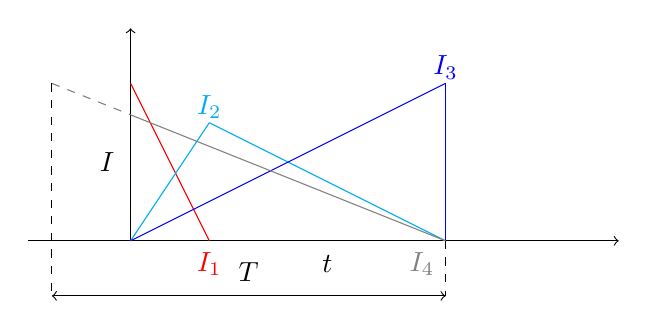
\begin{tikzpicture}
            %画x和y轴坐标
            \draw[<->](6.2,0)--(0,0)--(0,2.7);
            \draw[-](-1.3,0)--(0,0);

            \draw[red, domain=0:1] plot(\x, 2 - 2*\x) node at (1,-0.3){$I_1$};
            \draw[cyan, domain=0:1] plot(\x, 1.5 * \x) node at (1,1.7){$I_2$};
            \draw[cyan, domain=1:4] plot(\x, 2 - 0.5 * \x);
            \draw[blue, domain=0:4] plot(\x, 0.5 *\x) node at (4, 2.2){$I_3$};
            \draw[blue] (4, 2) -- (4, 0);
            \draw[gray, domain=0:4] plot(\x, 1.6 - 0.4*\x) node at (3.7, -0.3){$I_4$};
            \draw[gray, dashed, domain=-1:0] plot(\x, 1.6 - 0.4*\x);
            \draw node at (2.5, -0.3){$t$};
            \draw node at (-0.3, 1){$I$};

            \draw[dashed] (-1, 2) -- (-1, -0.7);
            \draw[dashed] (4, 0) -- (4, -0.7);
            \draw[<->] (-1, -0.7) -- (4, -0.7) node at (1.5, -0.4){$T$};

        \end{tikzpicture}
        \caption{一个周期内库存水平随时间变化曲线}
        \label{fig:multi-storage}
    \end{figure}
        
    \subparagraph*{b)} 根据图\ref{fig:multi-storage},一个周期内的单位启动成本

    \begin{align}
        c_k &= \frac{K_1 + K_2 + K_3}{Q} \\
        c_h &= \frac{Qh_1}{2p_1} + \frac{Q(p_1 - p_2)h_2}{2p_1p_2} + \frac{Qh_3}{2p_2} + \frac{Qh_4}{2d}
    \end{align}

    $G(Q) = c_k + c_h$,取最小值时满足$G'(Q^*) = 0$,此时

    \begin{equation}
        Q^* = \sqrt{\frac{2\left(K_1 + K_2 + K_3\right)}{\frac{h_1}{p_1} + \frac{h_2\left(p_1 - p_2\right)}{p_1p_2} + \frac{h_3}{p_2} + \frac{h_4}{d}}}
    \end{equation}

    此时,有$T^* = Q^*/d$,即

    \begin{equation}
        T^* = \left.\sqrt{\frac{2\left(K_1 + K_2 + K_3\right)}{\frac{h_1}{p_1} + \frac{h_2\left(p_1 - p_2\right)}{p_1p_2} + \frac{h_3}{p_2} + \frac{h_4}{d}}} \right/ d
    \end{equation}

    \separate
\end{document}